\customtitlepage{TemporalVLM: Video LLMs for Temporal Reasoning in Long Videos
}{Fawad J. Fateh, Umer Ahmed, Hamza Khan, M. Zeeshan Zia, Quoc-Huy Tran}

\section{TemporalVLM: Video LLMs for Temporal Reasoning in Long Videos}
\subsection{Abstract}

\begin{frame}{Abstract}
    \begin{block}{Proposed Solution}
        \texttt{TemporalVLM} is a video LLM model for temporal reasoning and fine-grained understanding in long videos. It inclues a \texttt{visual encoder} for mapping a long-term video into features which are \textbf{time-aware} and contain both \textbf{local} and \textbf{global} cues.

        \begin{itemize}
            \item Divide video into \textbf{short-term clips}, jointly encoded with \textit{timestamps} and \textbf{fused} across overlapping temporal windows.
            \item Local features are passed through \textbf{Bidirectional Long Short-term Memory (BiLSTM)} module for global feature aggeration.
            \item They also introduce a large-scale long video datasets. 
        \end{itemize}
    \end{block}
\end{frame}

\subsection{Pipeline}
\begin{frame}{Pipeline}
    \begin{figure}
        \centering
        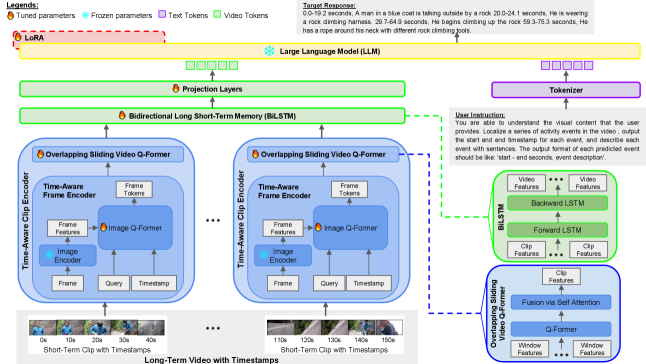
\includegraphics[width=0.75\textwidth]{img/general/temporalvlm_pipeline.png}
        \caption{TemporalVLM includes two novel components: a time-aware clip encoder for extracting time-aware fine-grained cues and a BiLSTM module for capturing long-range temporal dependencies.}
    \end{figure}
\end{frame}

\subsection{Contributions}
\begin{frame}{Contributions}
    \begin{block}{Short-Term Temporal Reasoing}
        They introduce a \textbf{time-aware} clip encoder for extracting fused local fine-grained cues within a clip. 
        \begin{itemize}
            \item Divide long-term video into short-term clips. Then \textbf{sampled frames} along with timestamps are then passed to \textbf{time-aware clip encoder} for jointly encoding frame contents and timestamps.
            \item They used a pre-trained image encoder to obtain frame features, which are jointly encoded with timestamps via an image \texttt{Q-Former}.
        \end{itemize}
    \end{block}
    \begin{block}{Long-Term Temporal Reasoning}
        \textbf{Bidirectional Long Short-Term Memory}, a module for computing global features across multiple clips. 
        \begin{itemize}
            \item Concatenate \textbf{time-aware} local features extracted from clips in temporal order.
            \item Pass the sequence of local features to the BiLSTM for aggerating global features. 
        \end{itemize}
    \end{block}
\end{frame}